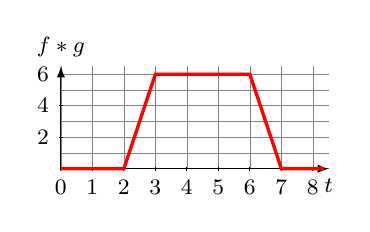
\begin{tikzpicture}
    [
    x=1cm, y=0.5cm, scale=0.4, font=\footnotesize, >=latex 
    %Voreinstellung für Pfeilspitzen
    ]
    
    %Raster im Hintergrund
    \draw[step=1, gray, very thin] (0,0) grid (8.5,6.5);
    
    %Zahlen auf x-Achse
    \foreach \x in {0,1,2,3,4,5,6,7,8}
    \draw[shift={(\x,0)},color=black] (0pt,2pt) -- (0pt,-2pt) node[below]
    {\footnotesize $\x$};
    
    %Länge x Achse
    \draw [-latex] (0,0) -- ++(8.5,0) node[below] {$t$};
    
    %Länge y Achse
    \draw [-latex] (0,0) -- ++(0,6.5) node[above] {$f*g$};
    
    %Zahlen auf y-Achse 
    %\foreach \y in {0,...,1}
    \foreach \y in {2,4,6}
    \draw[shift={(0,\y)},color=black] (2pt,0pt) -- (-2pt,0pt) node[left]
    {\footnotesize $\y$};
    
    %f(t)
    \draw[red, very thick] (0,0) -- (2,0) -- (3,6) -- (6,6) -- (7,0) -- (8.35,0); 
\end{tikzpicture}